%!TEX root = ../Thesis.tex

\section{Problem 2}
\label{sec:problem_2}%

The second 2D steady-state heat conduction problem we aim to address involves a square plate made of a thermally isotropic material, with a side length of 1 m and a negligible thickness of 1 mm. The temperature distribution $T=T(x,y)$ is specified along the entire boundary $\Gamma$, providing the necessary boundary conditions for the analysis. 

We are going to solve this problem using both MATLAB and Abaqus softwares. Specifically, we want to compare the solutions obtained from the FEM and the BEM at the nine internal nodes illustrated in the following figure:
\begin{figure}[H]
    \centering
    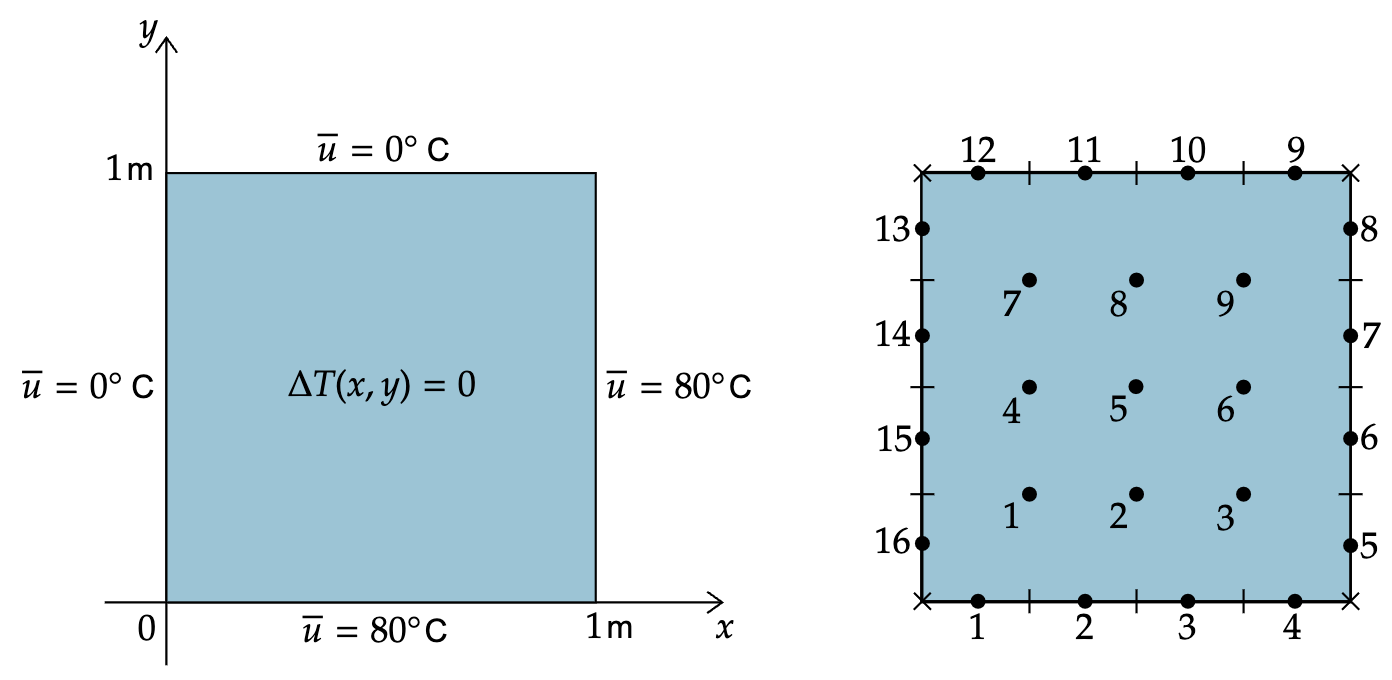
\includegraphics[width=0.8\textwidth]{pr2f1}
    \caption{Left: square domain $\Omega$ and boundary conditions of Problem 2. Right: boundary element discretization and internal points of Problem 2.}
    \label{fig:2pr2f1}
\end{figure}

\subsection{MATLAB Implementation}
\label{sub:MATLAB_implementation3}%

As we can see from the previous picture, the set up of this problem and Problem 1 are equal. Therefore, we simply run the script \texttt{main22} (Algorithm~\ref{alg:main22}), and we obtain the following output:
\begin{matlaboutput}
*********************************************************************
RESULTS
*********************************************************************

BOUNDARY NODES:

NODE        XM            YM            U             U_n
 1        0.12500       0.00000      80.00000     470.36316
 2        0.37500       0.00000      80.00000     116.43137
 3        0.62500       0.00000      80.00000      66.83419
 4        0.87500       0.00000      80.00000      18.38842
 5        1.00000       0.12500      80.00000      18.38842
 6        1.00000       0.37500      80.00000      66.83419
 7        1.00000       0.62500      80.00000     116.43137
 8        1.00000       0.87500      80.00000     470.36316
 9        0.87500       1.00000       0.00000    -470.36316
 10       0.62500       1.00000       0.00000    -116.43137
 11       0.37500       1.00000       0.00000     -66.83419
 12       0.12500       1.00000       0.00000     -18.38842
 13       0.00000       0.87500       0.00000     -18.38842
 14       0.00000       0.62500       0.00000     -66.83419
 15       0.00000       0.37500       0.00000    -116.43137
 16       0.00000       0.12500       0.00000    -470.36316

INTERNAL POINTS:

POINT        XIN           YIN           U
  1        0.25000       0.25000      40.00000
  2        0.50000       0.25000      57.88403
  3        0.75000       0.25000      69.15628
  4        0.25000       0.50000      22.11597
  5        0.50000       0.50000      40.00000
  6        0.75000       0.50000      57.88403
  7        0.25000       0.75000      10.84372
  8        0.50000       0.75000      22.11597
  9        0.75000       0.75000      40.00000
\end{matlaboutput}

\subsection{MATLAB scripts}
\label{sub:matlab_scripts3}%

\begin{matlab}{main22}{alg:main22}
%% Problem 2 - 2D steady state heat conduction problem
clear; clc; 

% Set the maximum dimensions
N = 16;
IN = 9;

% Set data
XL = [0; 0.25; 0.5; 0.75; 1; 1; 1; 1; 1; 0.75; 0.5; 0.25; 0; 0; 0; 0];
YL = [0; 0; 0; 0; 0; 0.25; 0.5; 0.75; 1; 1; 1; 1; 1; 0.75; 0.5; 0.25];
XIN = [0.25; 0.5; 0.75; 0.25; 0.5; 0.75; 0.25; 0.5; 0.75];
YIN = [0.25; 0.25; 0.25; 0.5; 0.5; 0.5; 0.75; 0.75; 0.75];
INDEX = zeros(N,1);
UB = zeros(N,1); UB(1:8) = 80;

% Compute midpoints
[XM, YM] = MIDPOINTS(XL, YL, N);


% Print data
INPUT(XL, YL, XM, YM, XIN, YIN, INDEX, UB, N, IN);

% Compute the G matrix
G = GMATR(XL, YL, XM, YM, N);

% Compute the H matrix
H = HMATR(XL, YL, XM, YM, N);

% Form the system of equations AX=B
[A, UNB] = ABMATR(G, H, UB, INDEX);

% Solve the system of equations
UNB = A\UNB;

% Form the vectors U and UN of all the boundary values
[UB, UNB] = REORDER(UB, UNB, INDEX);

% Compute the values UIN of u at the internal points
UIN = UINTER(XL, YL, XIN, YIN, UB, UNB, N, IN);

% Print results
OUTPUT(XM, YM, XIN, YIN, UB, UNB, UIN, N, IN);

\end{matlab}

\newpage

\subsection{Abaqus Implementation}
\label{sub:Abaqus_implementation3}%

In this section we solve Problem 2 through the Abaqus Software. The chosen units of measure are mm for length, °C for temperature, and W for power (energy per unit time). Consequently, the thermal conductivity of the material is given by:
\begin{equation}
\label{eq:conductivity}
k=1\ \frac{\text{W}}{\text{m °C}}=1000\ \frac{\text{W}}{\text{mm °C}}
\end{equation}

\subsubsection{Part module}

We analyze the plate as a 2D planar deformable shell body of size 2000:
\begin{figure}[H]
    \centering
    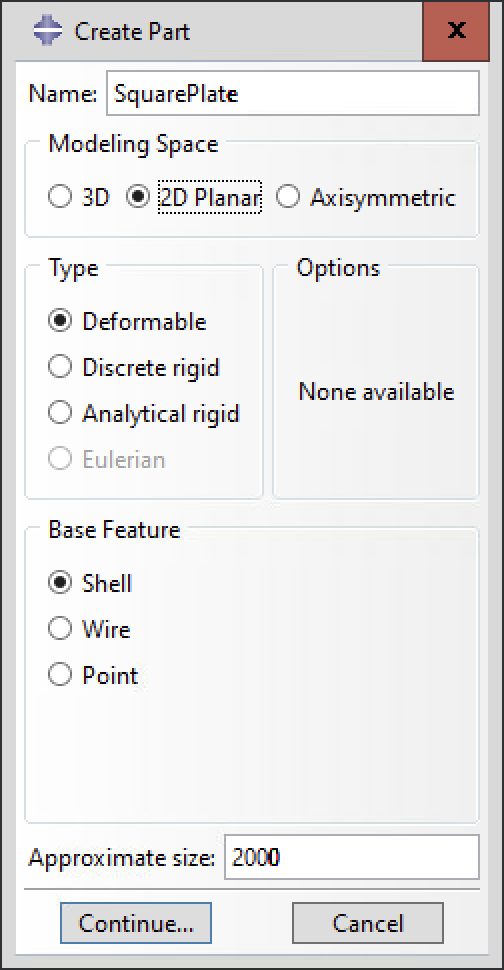
\includegraphics[width=0.2\textwidth]{Images/ab2/ab1.png}
    \caption{Create part.}
    \label{fig:ab1}
\end{figure}

We obtain:
\begin{figure}[H]
    \centering
    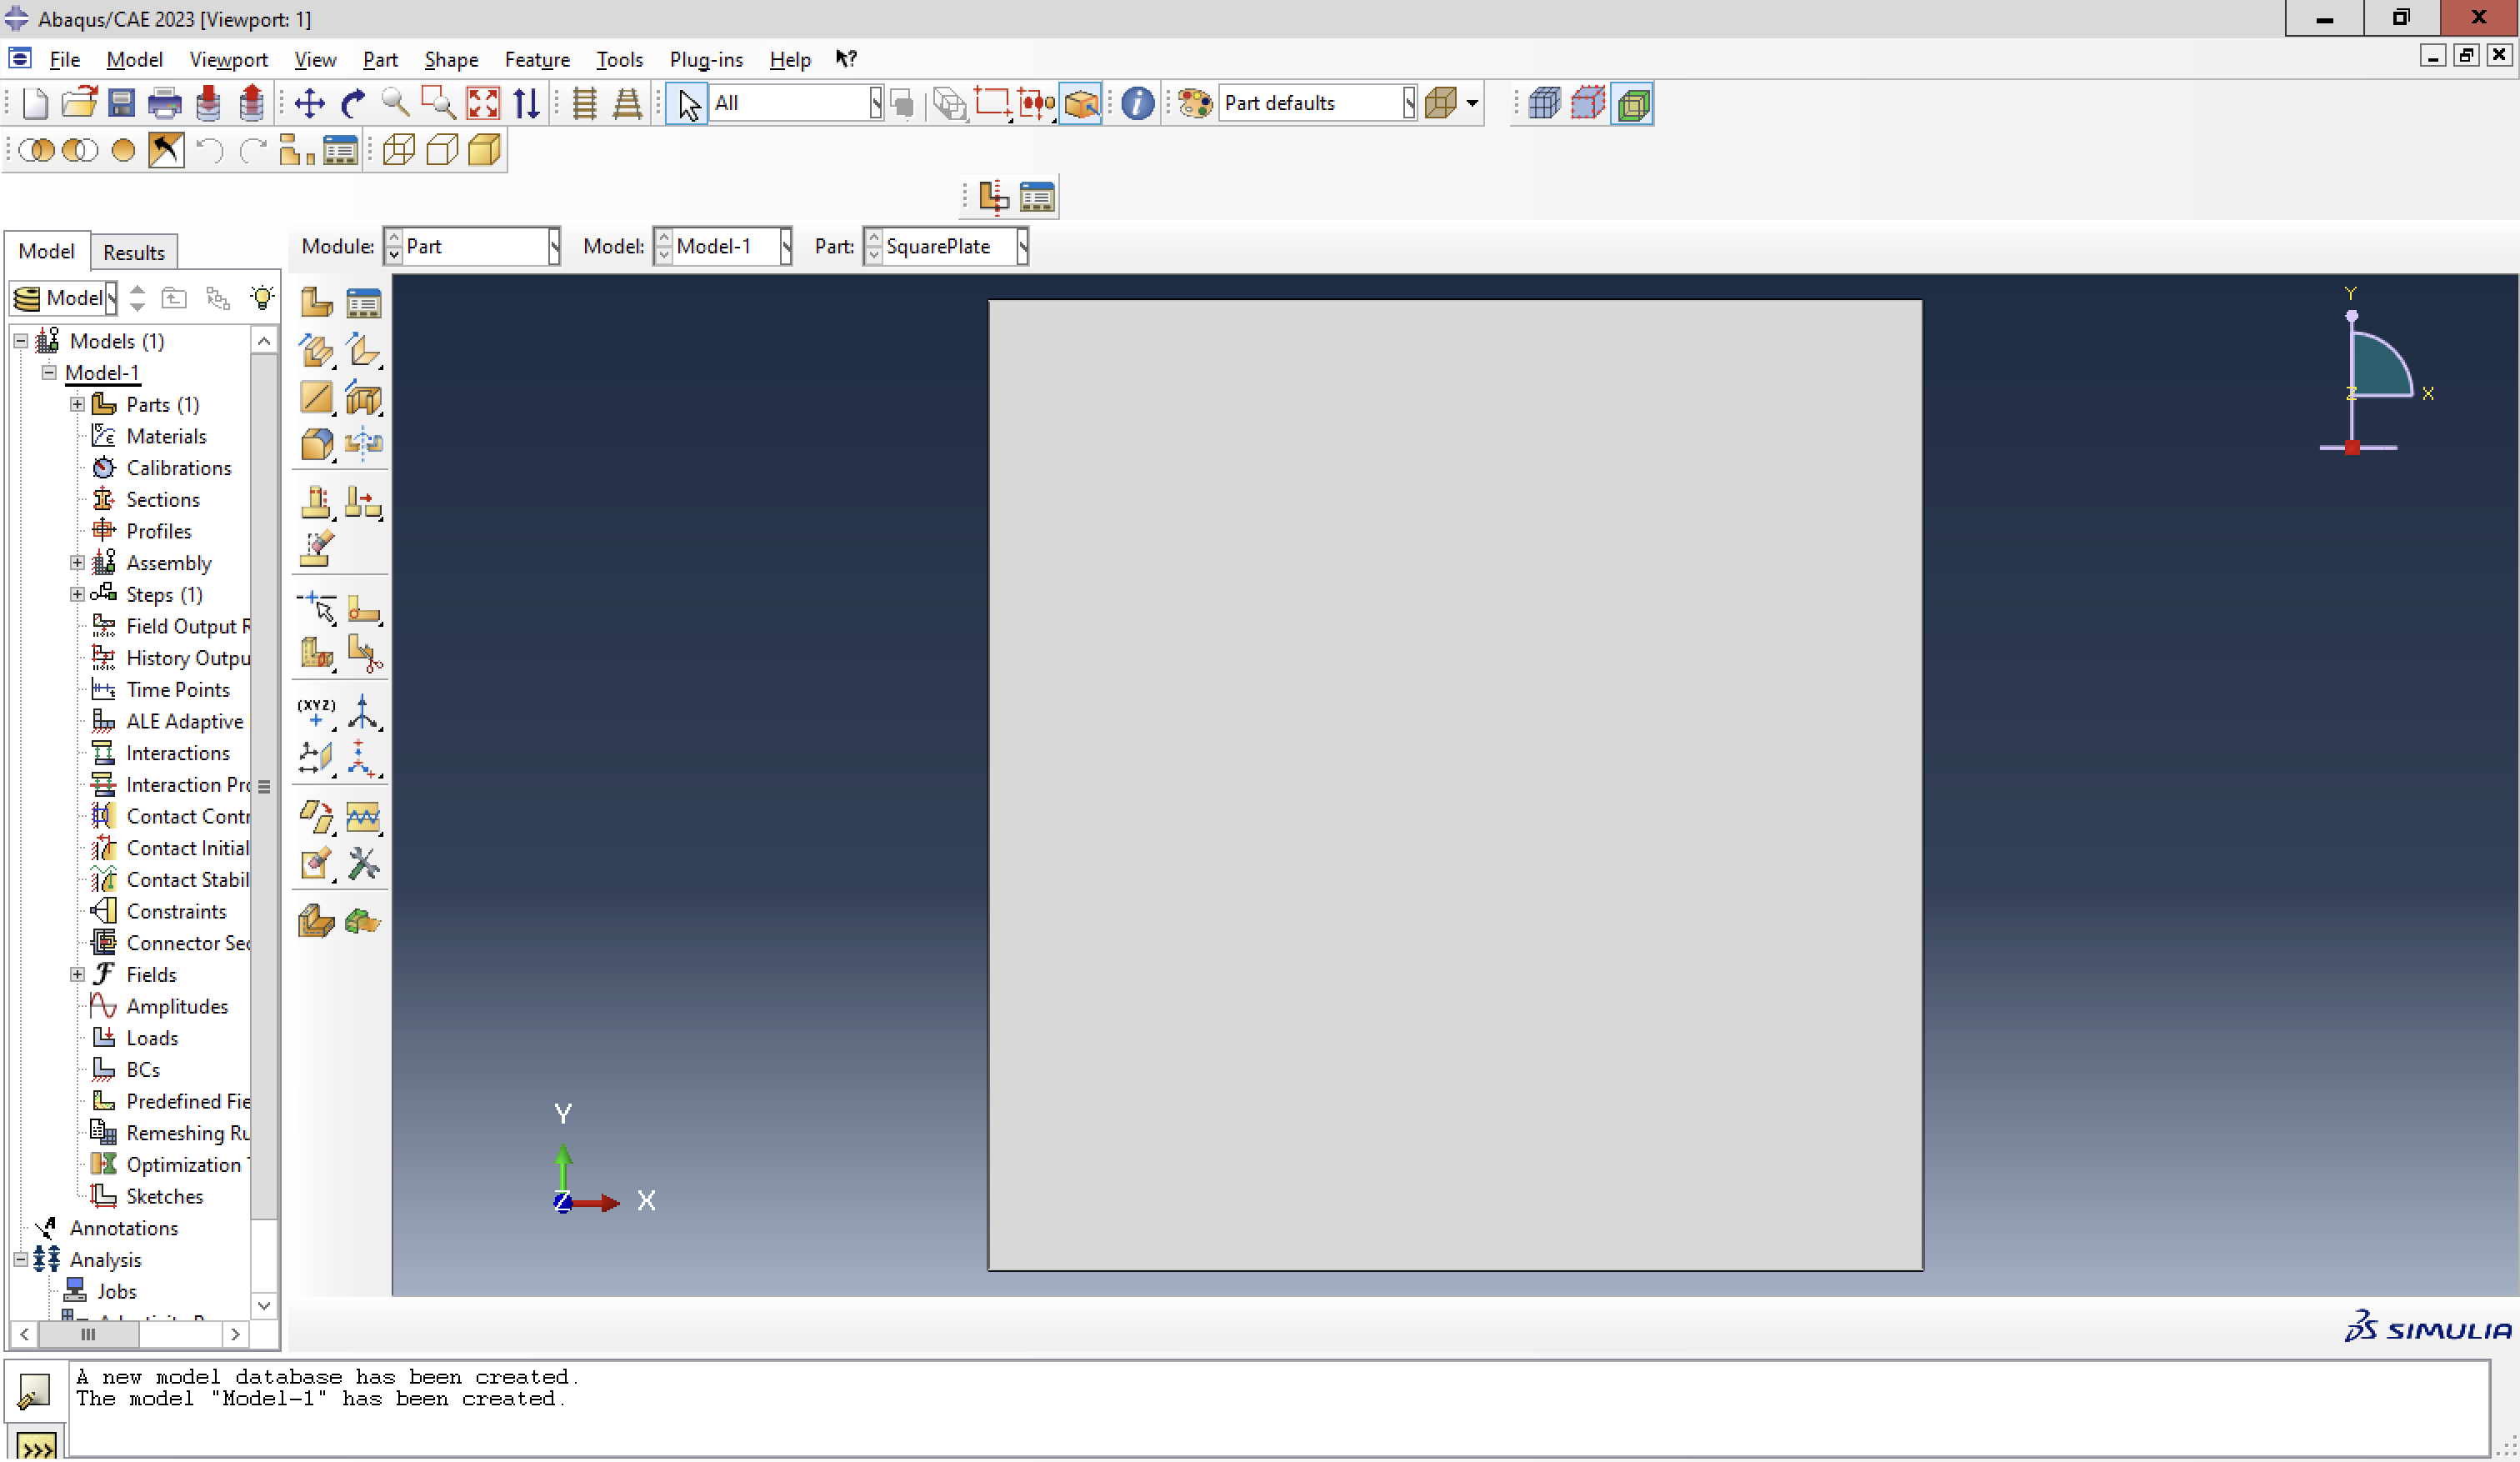
\includegraphics[width=0.8\textwidth]{Images/ab2/ab2.png}
    \caption{Final result of Part module.}
    \label{fig:ab2}
\end{figure}

\subsubsection{Property module}

We create a new material with conductivity $k$:
\begin{figure}[H]
    \centering
    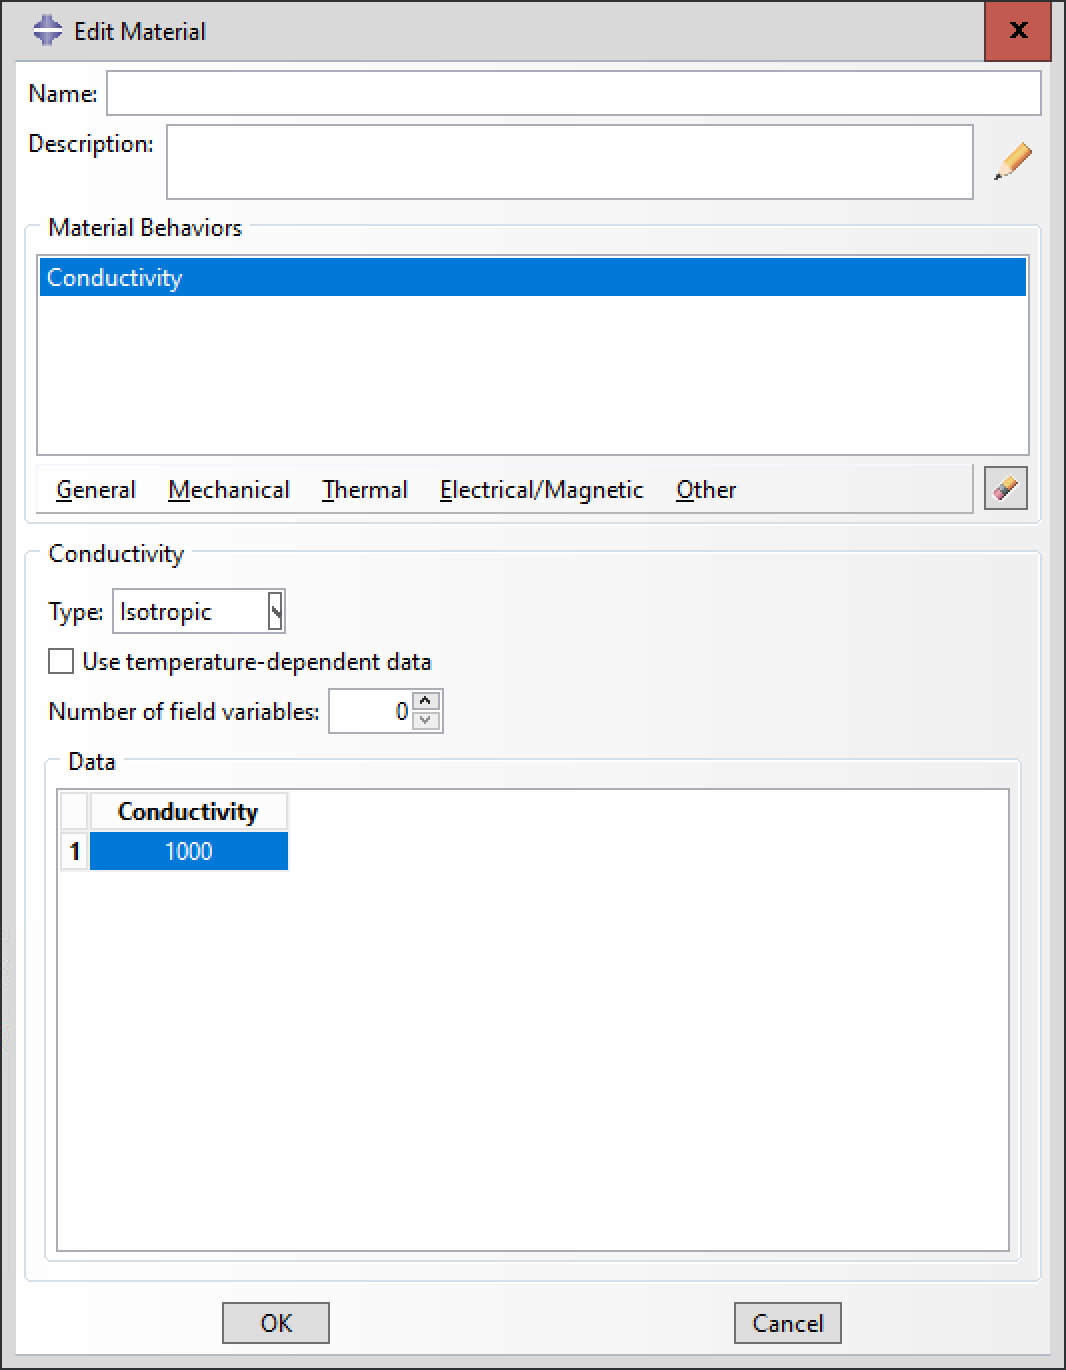
\includegraphics[width=0.35\textwidth]{Images/ab2/ab3.png}
    \caption{Create Material.}
    \label{fig:ab3}
\end{figure}

Then we define a solid and homogeneous section
\begin{figure}[H]
    \centering
    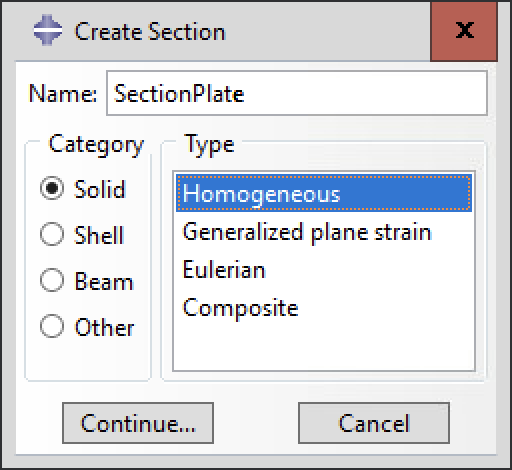
\includegraphics[width=0.25\textwidth]{Images/ab2/ab4.png}
    \caption{Create Section.}
    \label{fig:ab4}
\end{figure}

and we assign the section by selecting the whole plate, as Figure~\ref{fig:ab5} shows.

\begin{figure}[H]
    \centering
    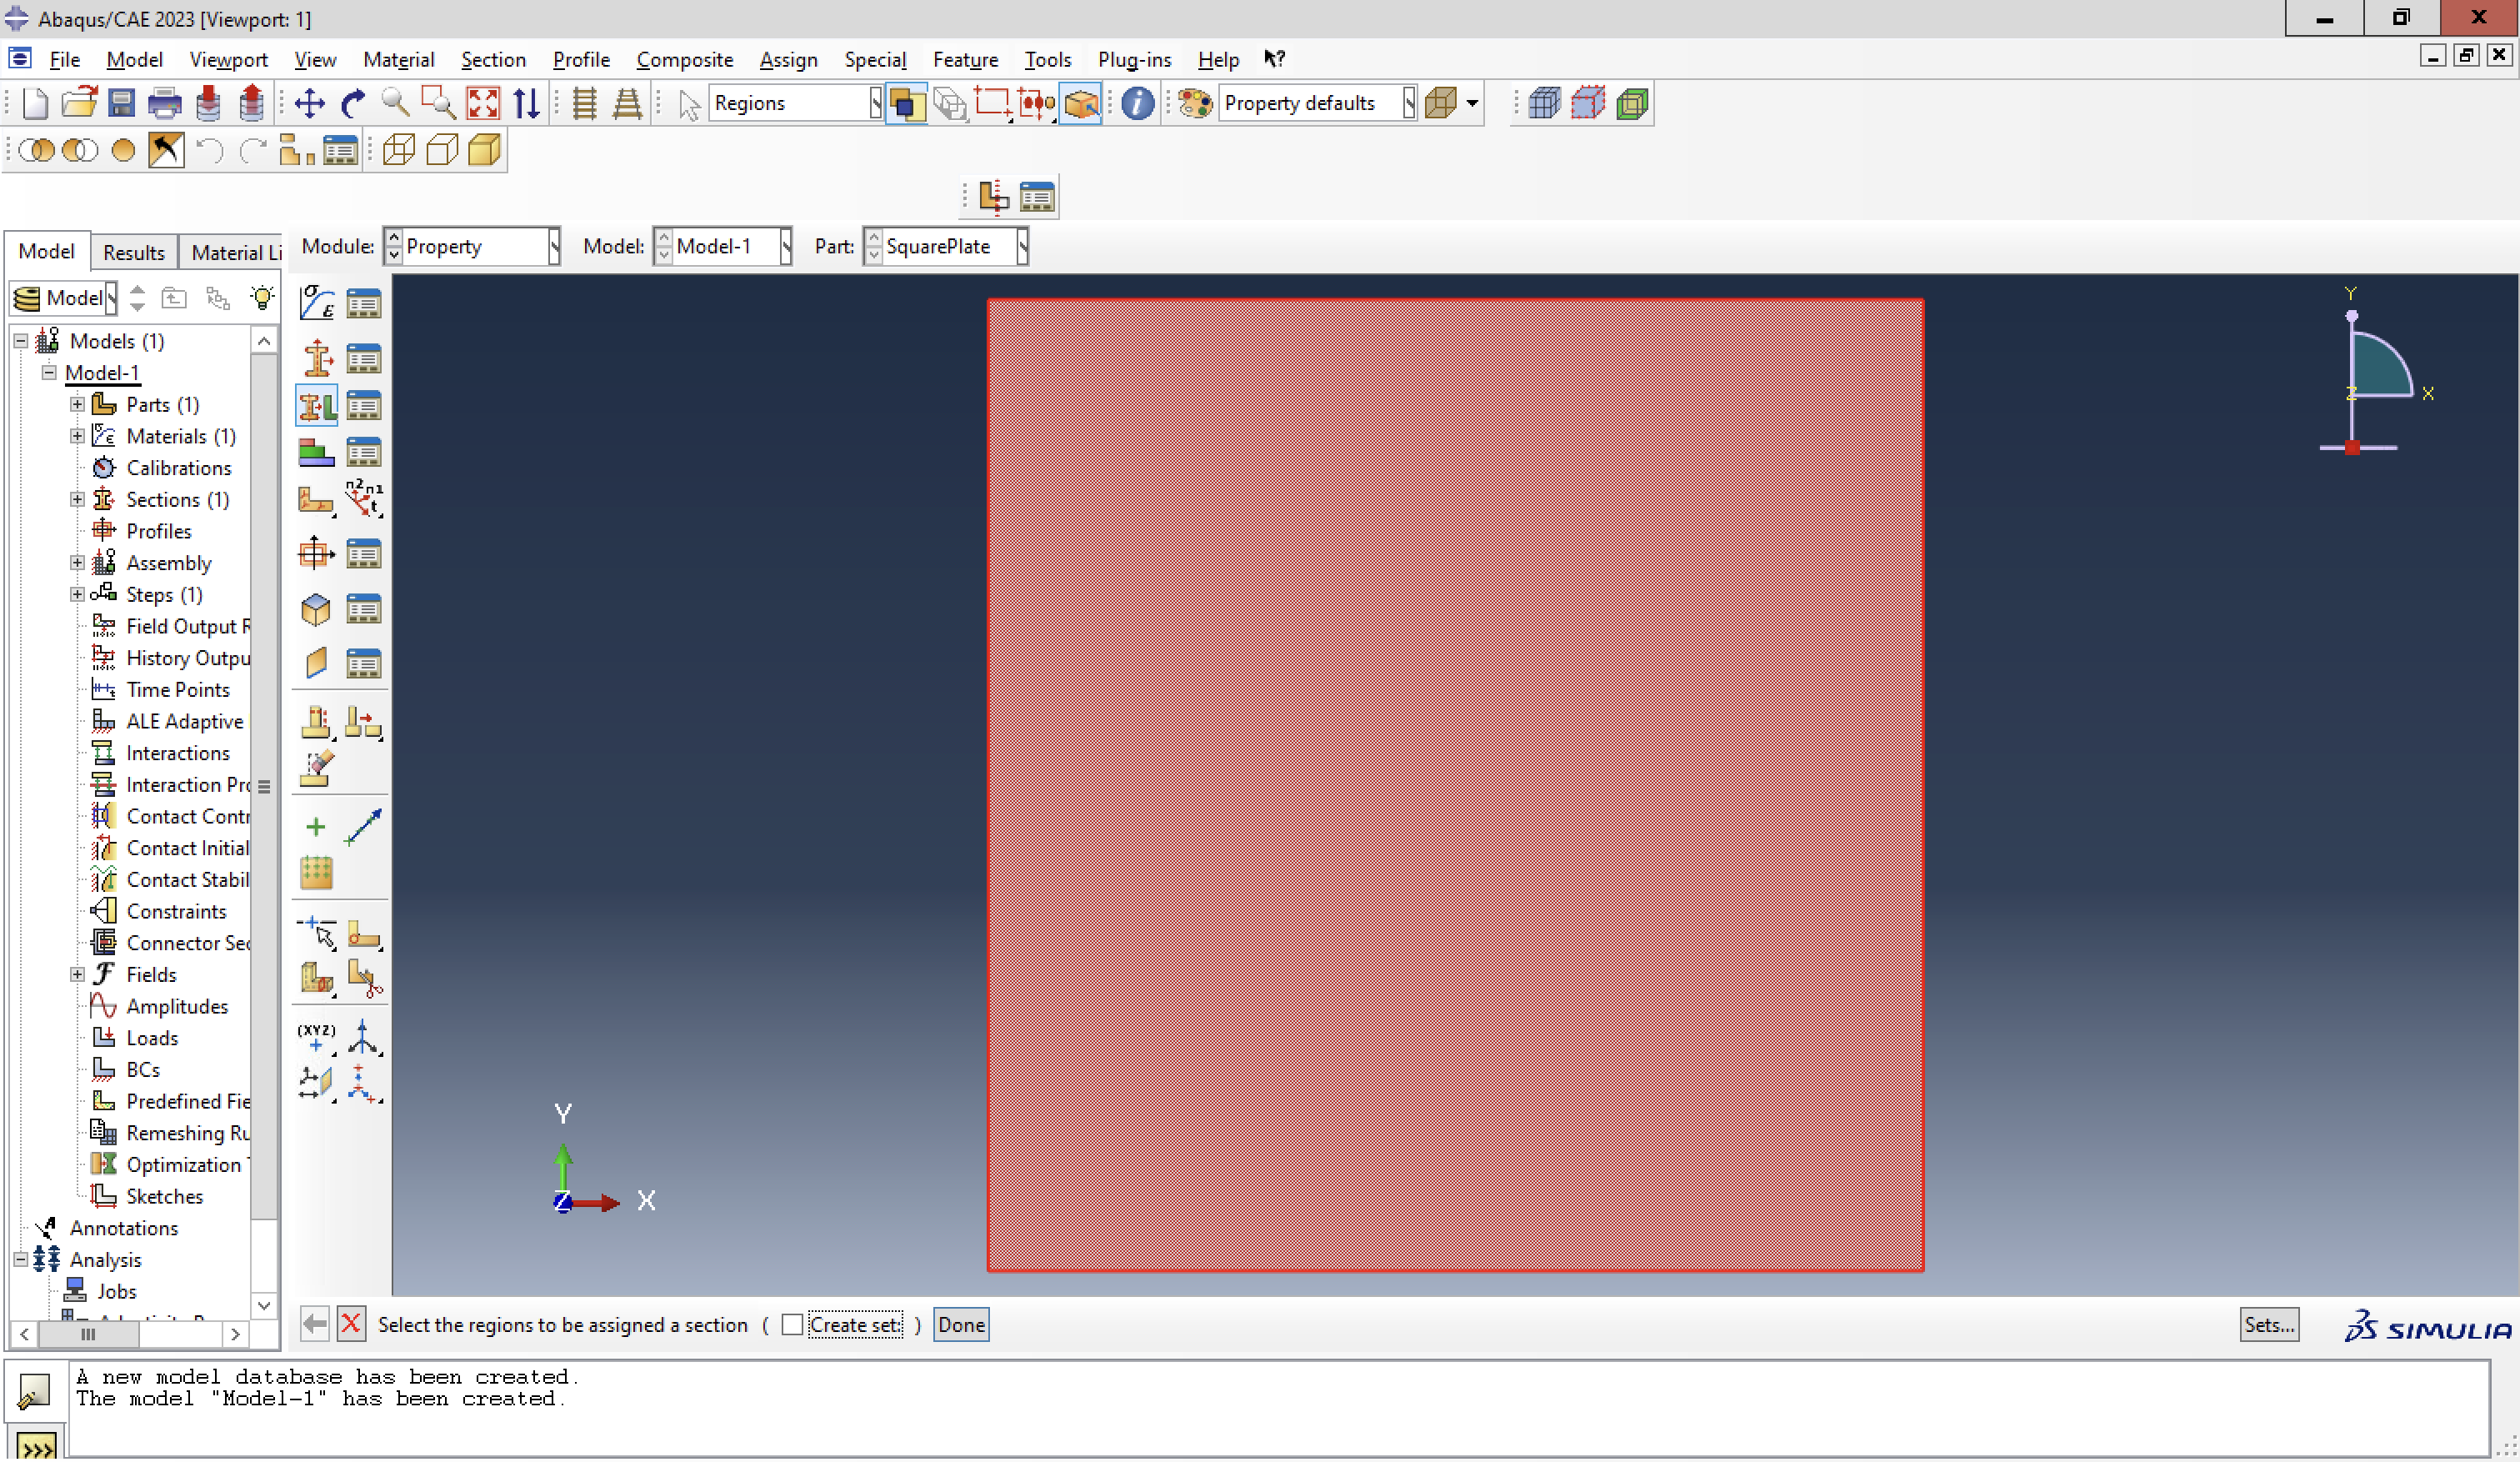
\includegraphics[width=0.9\textwidth]{Images/ab2/ab5.png}
    \caption{Assign Section.}
    \label{fig:ab5}
\end{figure}

\subsubsection{Assembly module}

Geometry and material have been defined at this stage. However, we need to create a dependent instance in order to apply boundary conditions:
\begin{figure}[H]
    \centering
    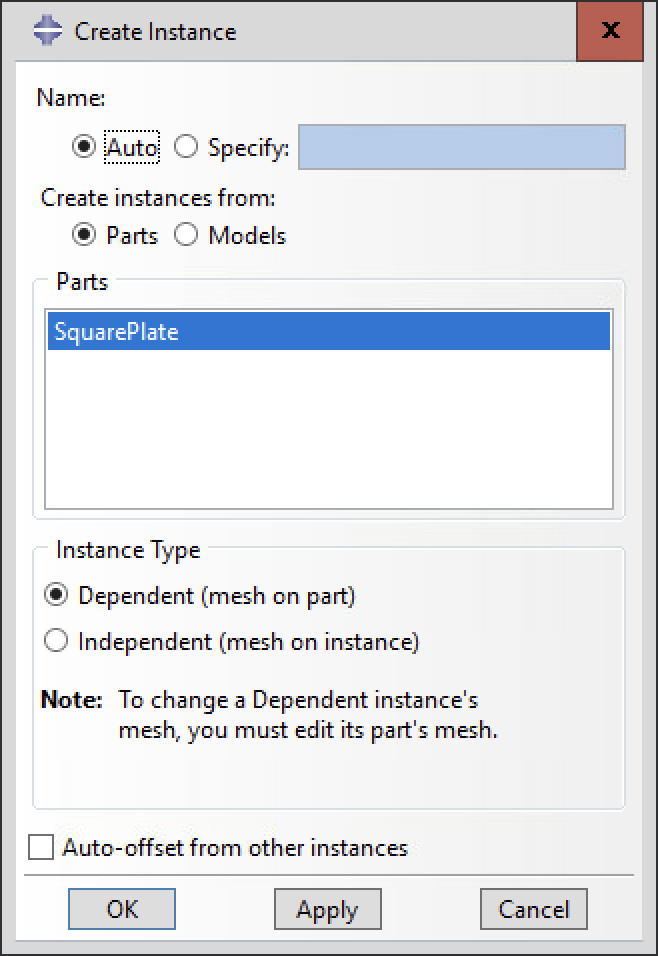
\includegraphics[width=0.3\textwidth]{Images/ab2/ab6.png}
    \caption{Create Instance.}
    \label{fig:ab6}
\end{figure}

Thus we get:
\begin{figure}[H]
    \centering
    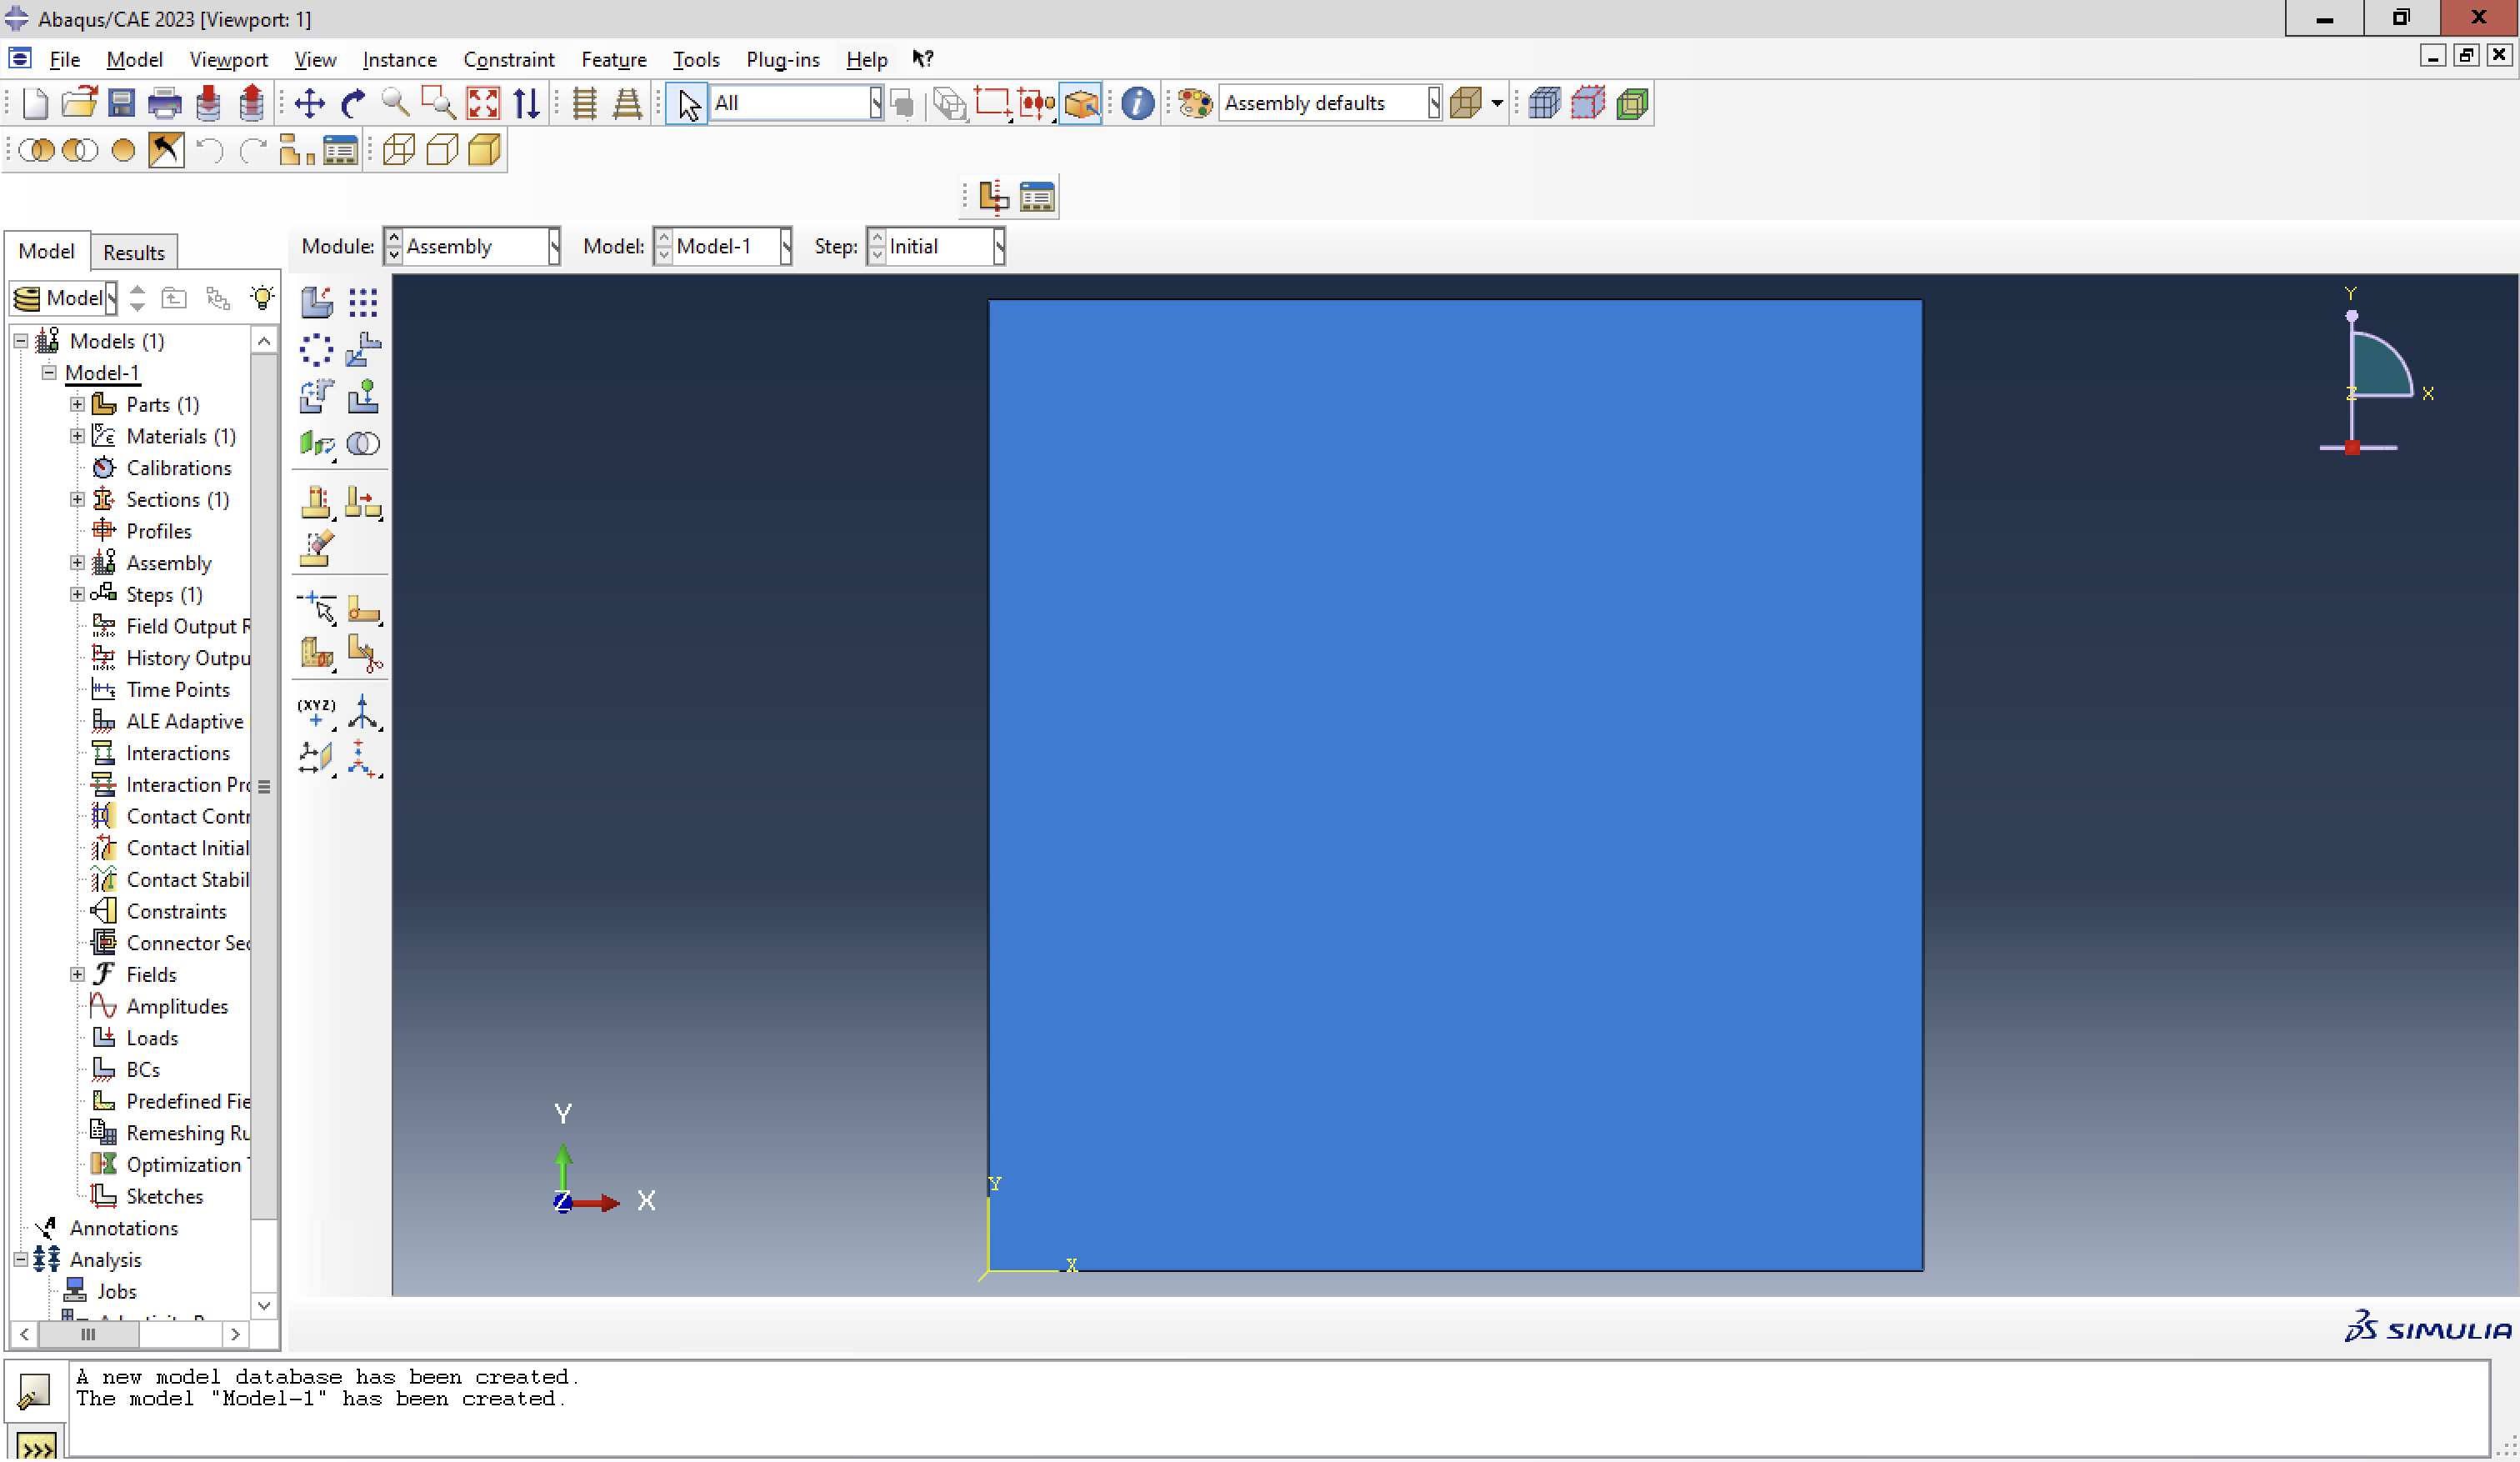
\includegraphics[width=1\textwidth]{Images/ab2/ab7.png}
    \caption{Final result of Assembly module.}
    \label{fig:ab7}
\end{figure}

\subsubsection{Step module}

In this module we define the type of analysis we need: a steady state heat transfer step.
\begin{figure}[H]
    \centering
    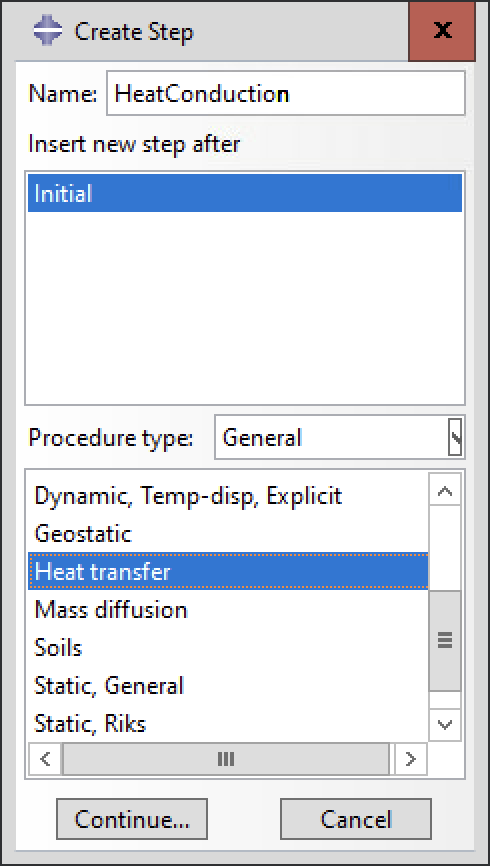
\includegraphics[width=0.275\textwidth]{Images/ab2/ab8.png} \qquad
    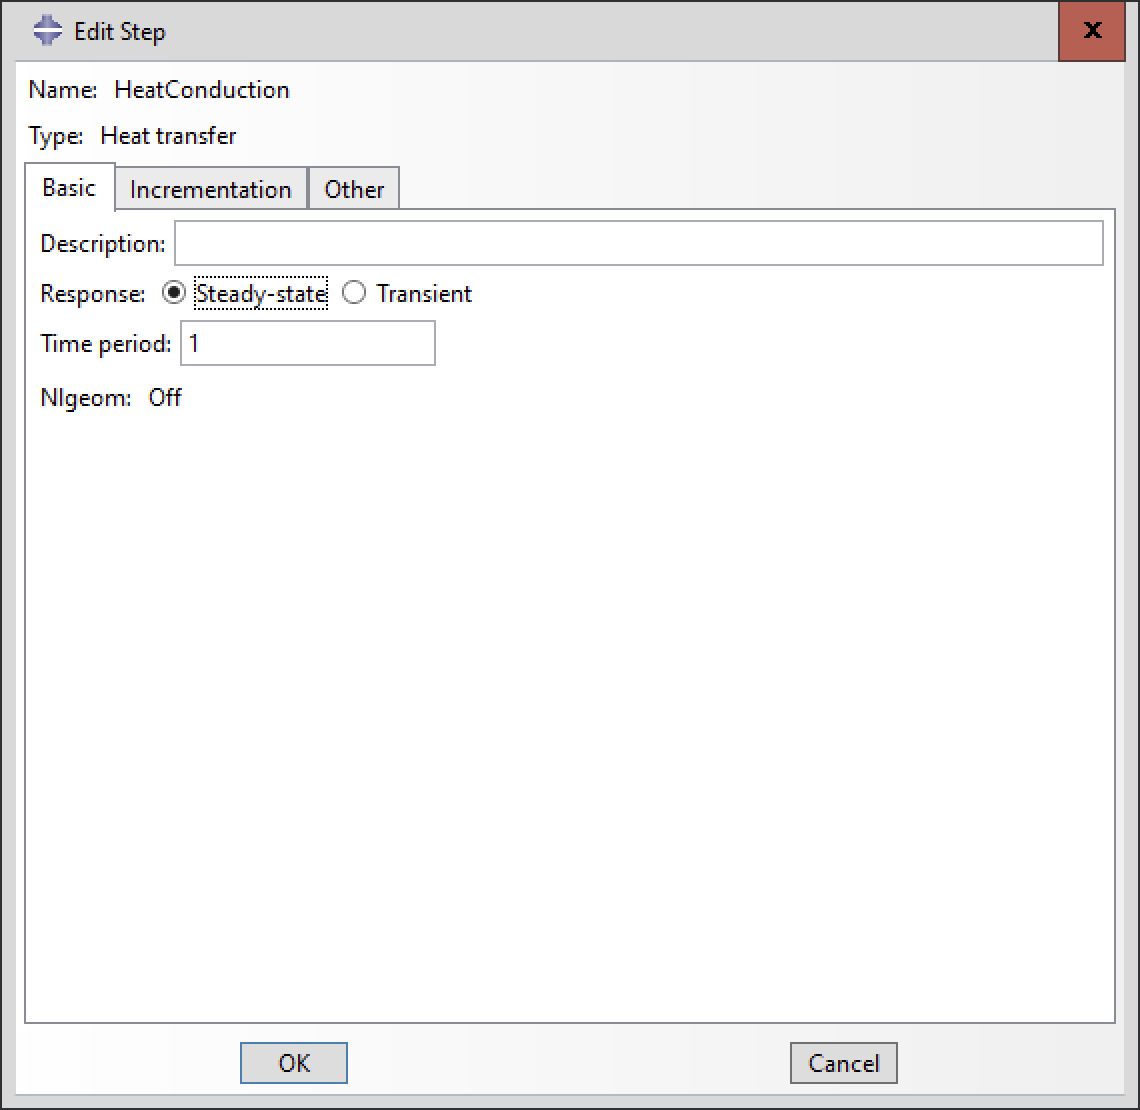
\includegraphics[width=0.5\textwidth]{Images/ab2/ab9.png}
    \caption{Create and edit step: heat transfer steady state analysis.}
    \label{fig:ab89}
\end{figure}

\newpage

\subsubsection{Load module}

We create the two different boundary conditions to be imposed on $\Gamma$:
\begin{figure}[H]
    \centering
    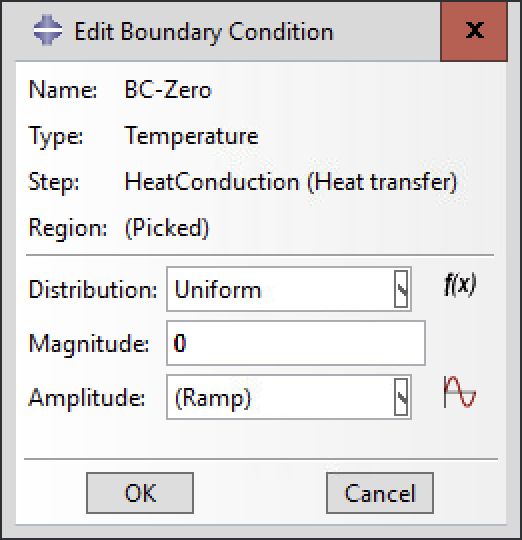
\includegraphics[width=0.3\textwidth]{Images/ab2/ab10.png} \qquad
    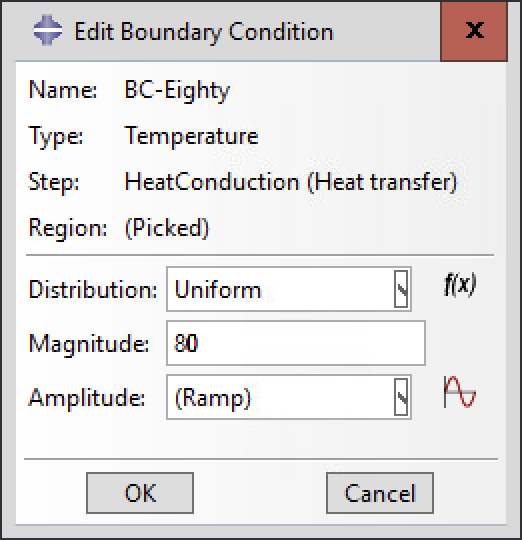
\includegraphics[width=0.3\textwidth]{Images/ab2/ab11.png}
    \caption{Create and edit boundary conditions.}
    \label{fig:ab1011}
\end{figure}

\begin{figure}[H]
    \centering
    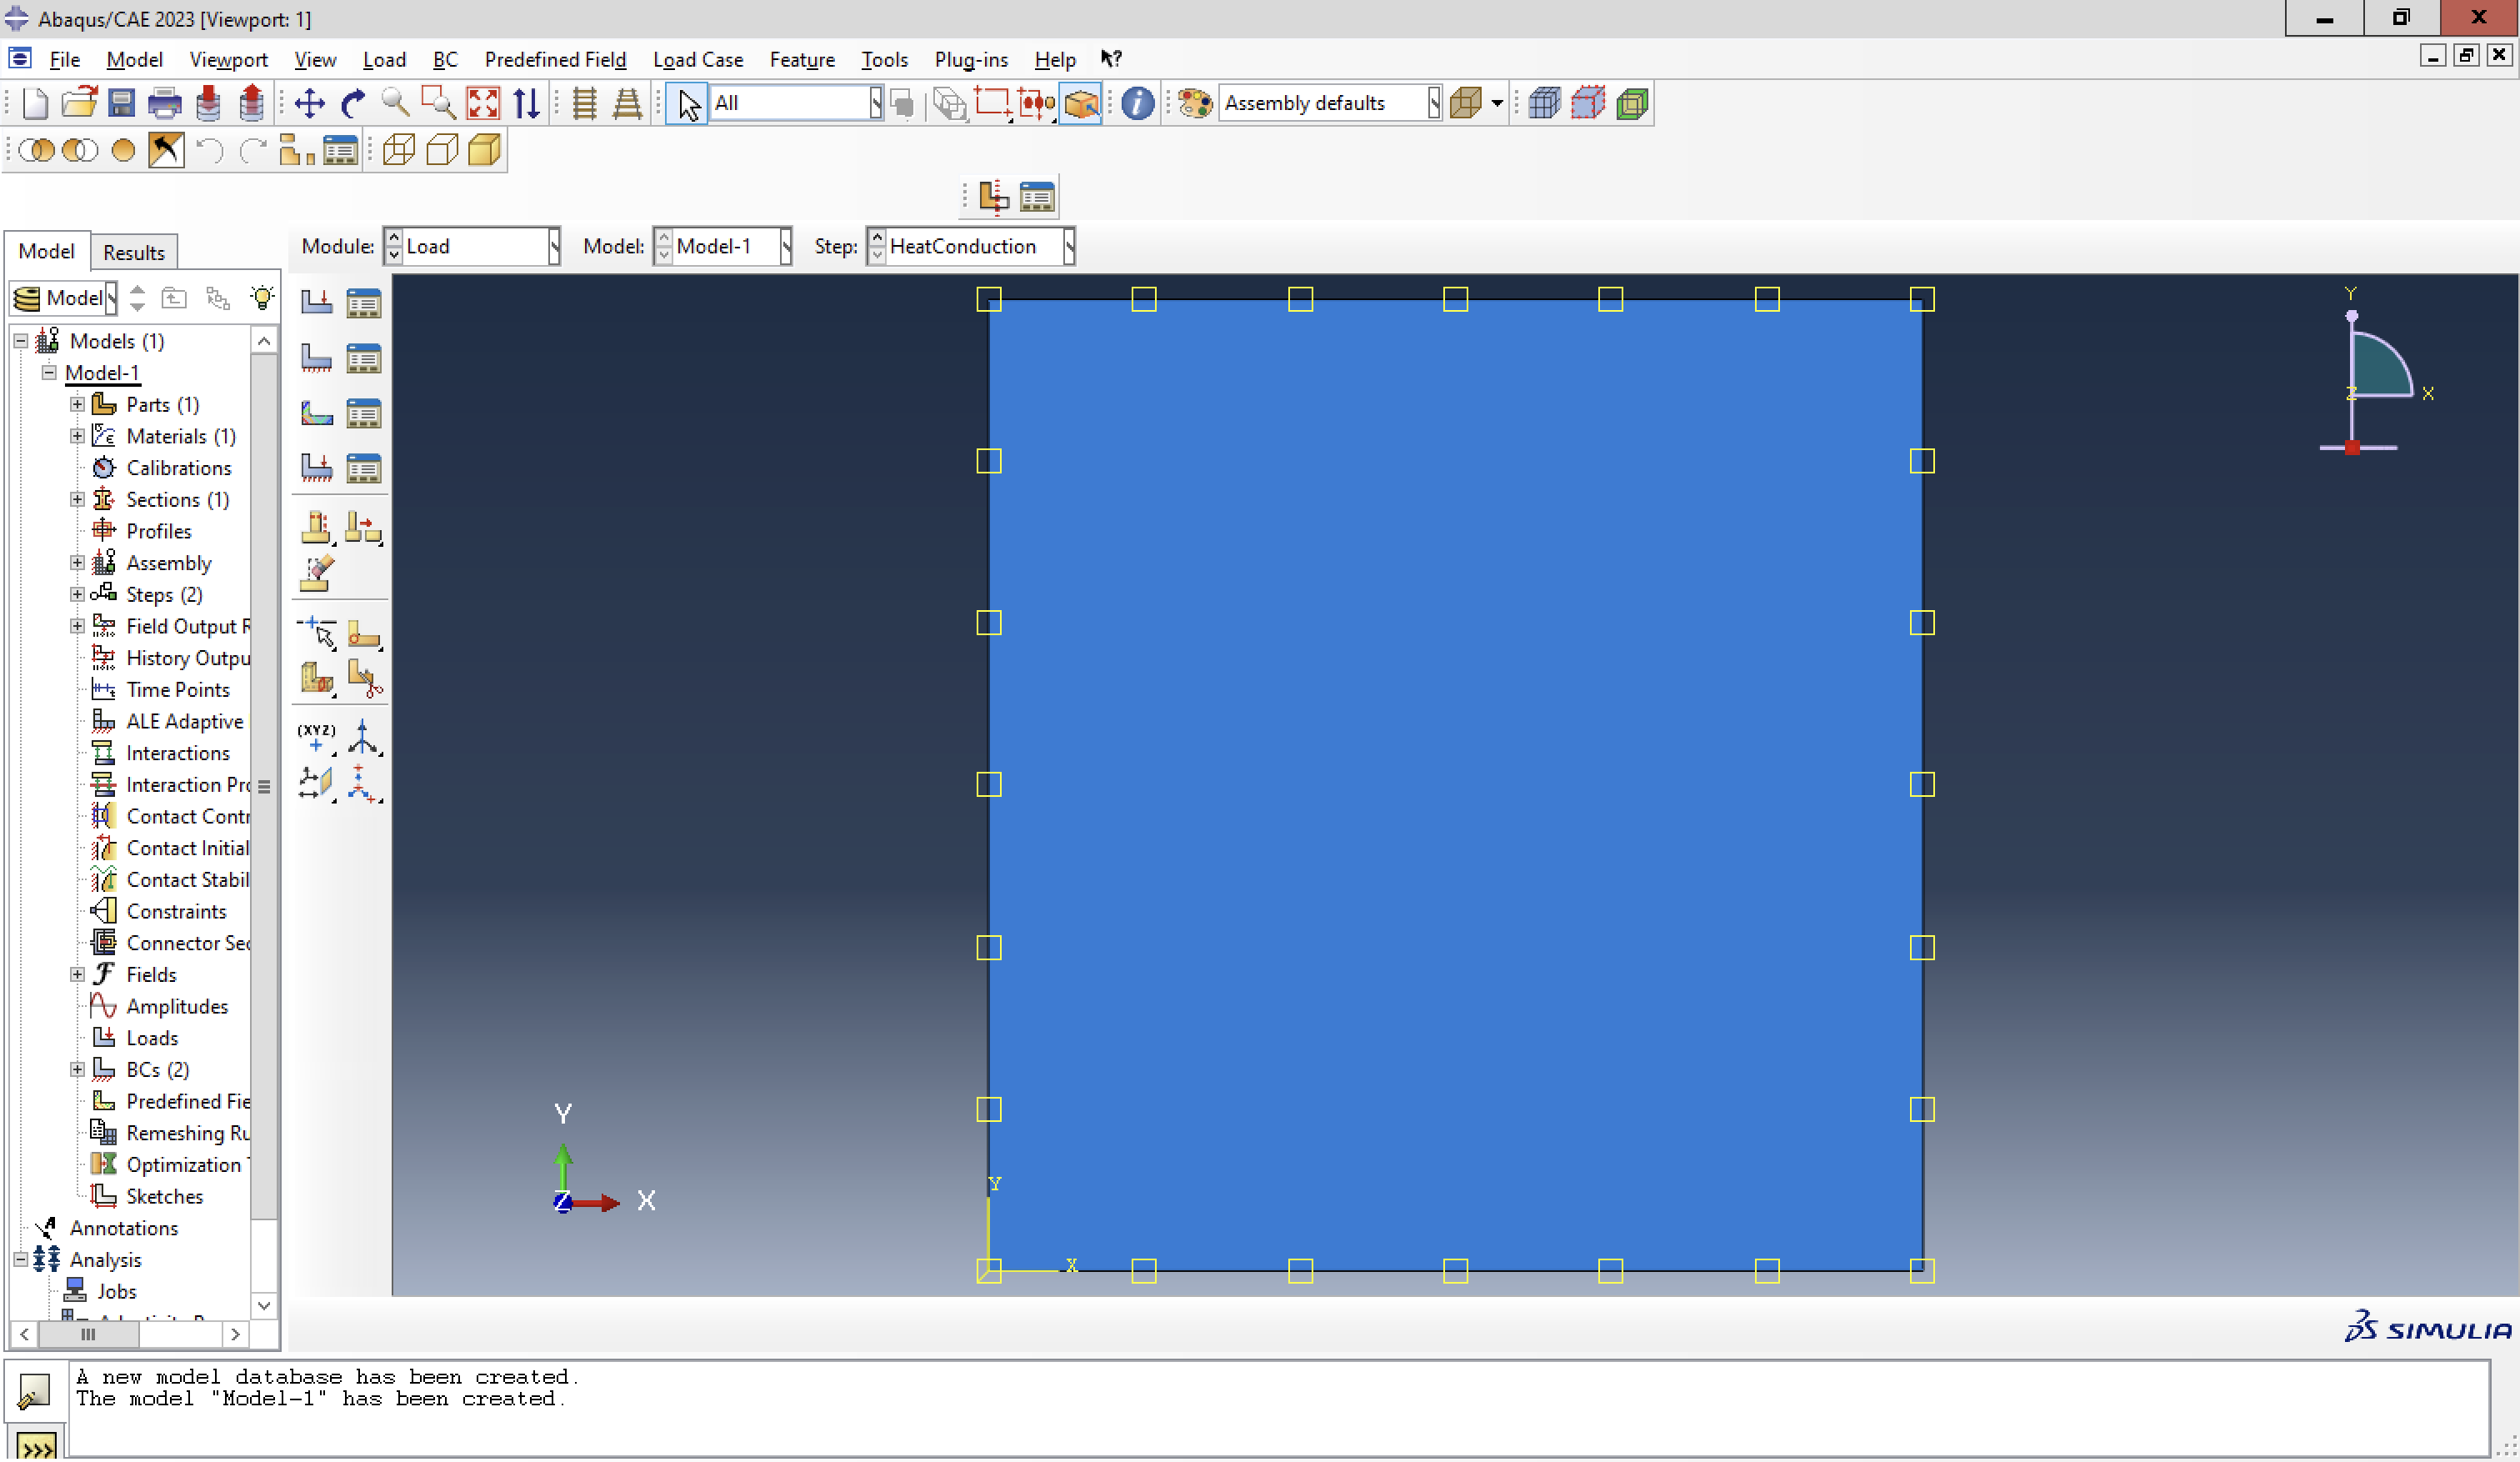
\includegraphics[width=\textwidth]{Images/ab2/ab12.png}
    \caption{Final result of Load module.}
    \label{fig:ab12}
\end{figure}

\newpage

\subsubsection{Mesh module}

Here we generate a mesh of 64 four-node linear heat transfer quadrilateral finite elements:
\begin{figure}[H]
    \centering
    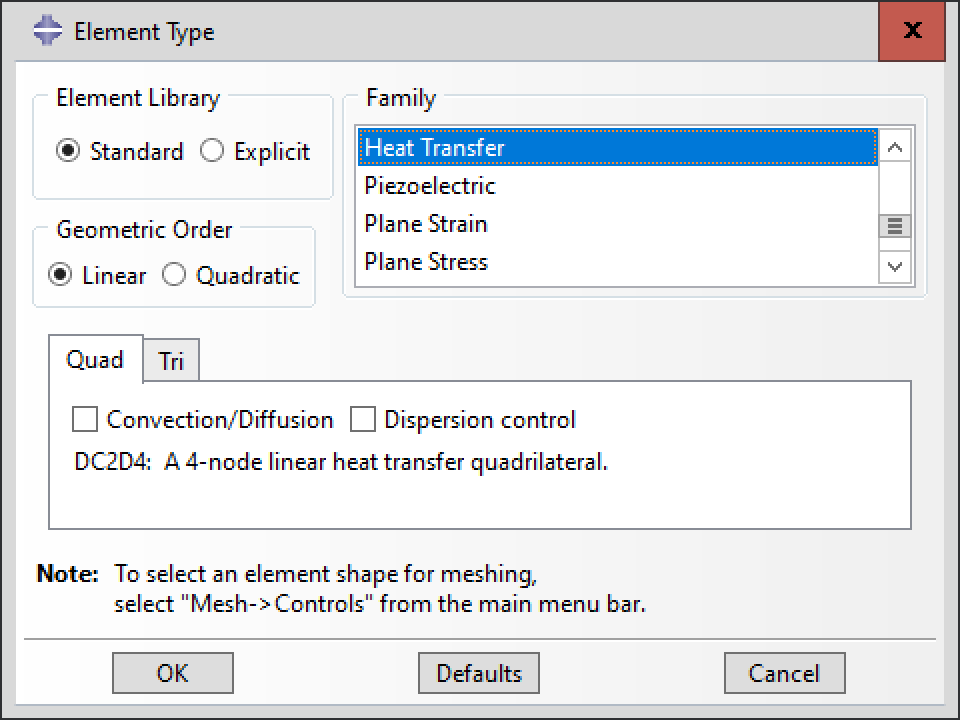
\includegraphics[width=0.5\textwidth]{Images/ab2/ab13.png} \qquad
    
\includegraphics[width=0.37\textwidth]{Images/ab2/ab14.png}
    \caption{Element type and generated mesh.}
    \label{fig:ab1314}
\end{figure}

\subsubsection{Job module} 

Finally, we can submit a standard job:
\begin{figure}[H]
    \centering
    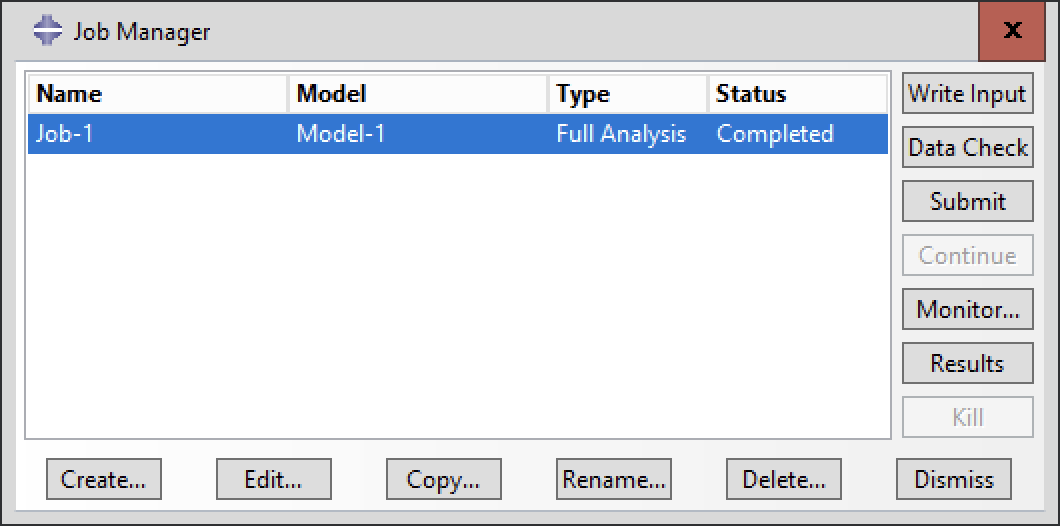
\includegraphics[width=0.6\textwidth]{Images/ab2/ab15.png}
    \caption{Job Manager.}
    \label{fig:ab15}
\end{figure}

\newpage

\subsubsection{Visualization module}

Results of the FEM analysis can be visualized in this module. We frist display the nodal temperature (NT11) distribution:
\begin{figure}[H]
    \centering
    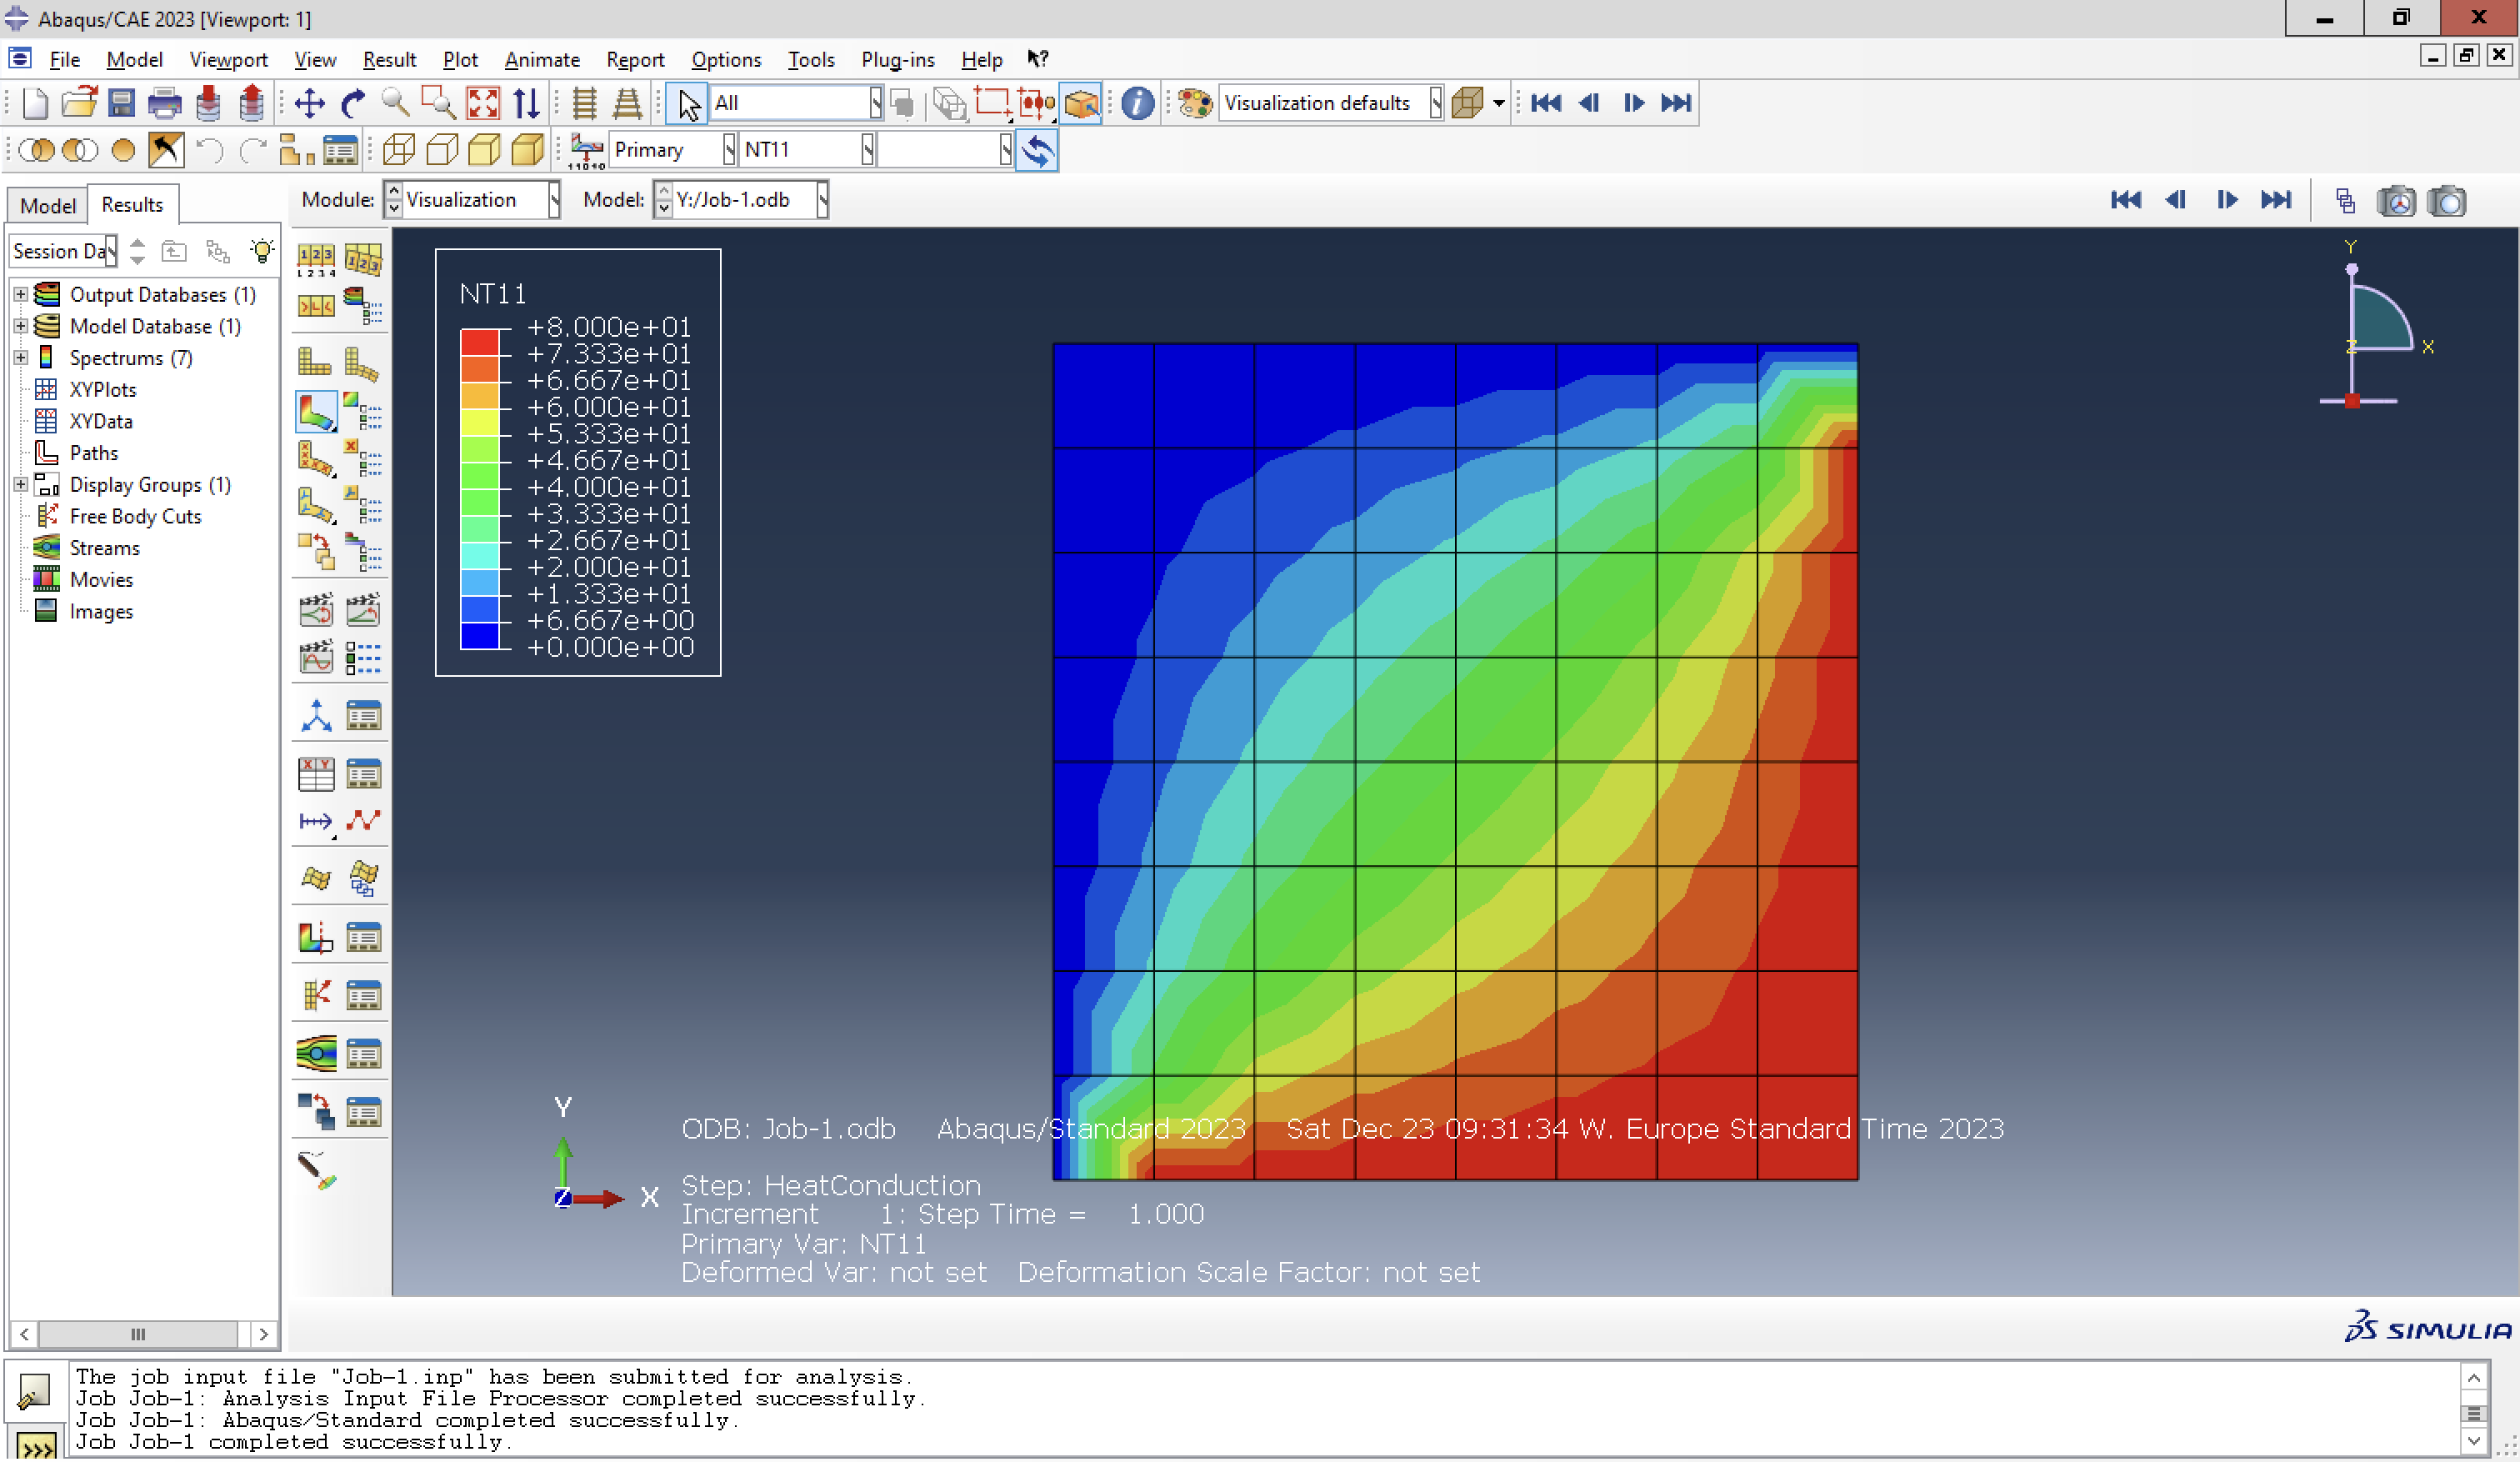
\includegraphics[width=\textwidth]{Images/ab2/ab16.png}
    \caption{Nodal temperature.}
    \label{fig:ab16}
\end{figure}

Then we proceed by selecting the nodal temperature of the nine internal node we are interested in:

\begin{figure}[H]
    \centering
    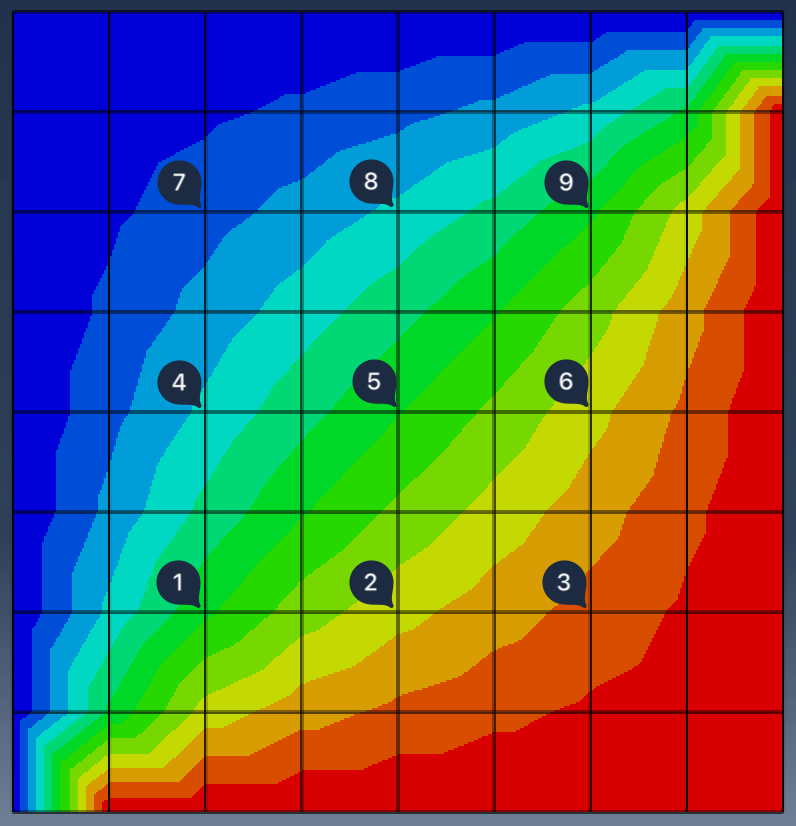
\includegraphics[width=0.4\textwidth]{Images/ab2/ab18.png} \qquad
    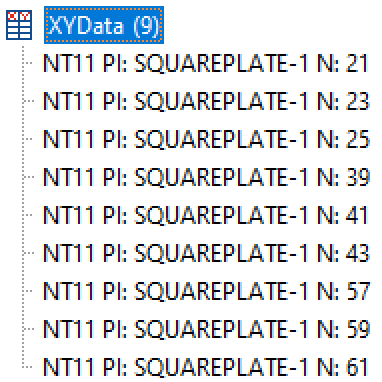
\includegraphics[width=0.4\textwidth]{Images/ab2/ab17.png}
    \caption{Nodal temperature of internal points.}
    \label{fig:ab1817}
\end{figure}

The numerical values are contained in Table~\ref{table:stedyRes}.

\subsection{Comparison between MATLAB and Abaqus}
\label{sub:comparison3}%

We now present the comparison of the results obtained from solving Problem 2 using MATLAB and Abaqus software. Both the Finite Element Method and the Boundary Element Method were employed to analyze the steady state heat conduction in a square plate with specified boundary conditions. The comparison focuses on the temperature distribution at nine selected internal nodes, as depicted in Fig.~\ref{fig:2pr2f1} and Fig.~\ref{fig:ab1817}:

\begin{table}[H]
    %\caption*{\textbf{Title of Table (optional)}}
    \centering 
    \begin{tabular}{ccccc}
    \hline
    \rowcolor{bluepoli!40} % comment this line to remove the color
    Internal Point label & Abaqus label & Abaqus value & MATLAB value & UoM \\
    \hline
    1 & NT11 N:21 & 38.6765 & 40.00000 & °C \\
    2 & NT11 N:23 & 57.6329 & 57.88403 & °C \\
    3 & NT11 N:25 & 69.0987 & 69.15628 & °C \\
    4 & NT11 N:39 & 21.5550 & 22.11597 & °C \\
    5 & NT11 N:41 & 39.5222 & 40.00000 & °C \\
    6 & NT11 N:43 & 57.6329 & 57.88403 & °C \\
    7 & NT11 N:57 & 10.5401 & 10.84372 & °C \\
    8 & NT11 N:59 & 21.5550 & 22.11597 & °C \\
    9 & NT11 N:61 & 38.6765 & 40.00000 & °C \\
    \hline
    \end{tabular}
    \\[10pt]
    \caption{Nodal temperature results of Problem 2.}
    \label{table:stedyRes}
\end{table}

The results presented in Table~\ref{table:stedyRes} demonstrate that the temperature values obtained from Abaqus and MATLAB are remarkably similar, indicating that the BEM maintains high accuracy while offering significant computational efficiency advantages over the FEM. 

Additionally, the results highlight a clear line of symmetry in the temperature distribution, which is consistent with the boundary conditions and the geometry of the problem:
\begin{figure}[H]
    \centering
    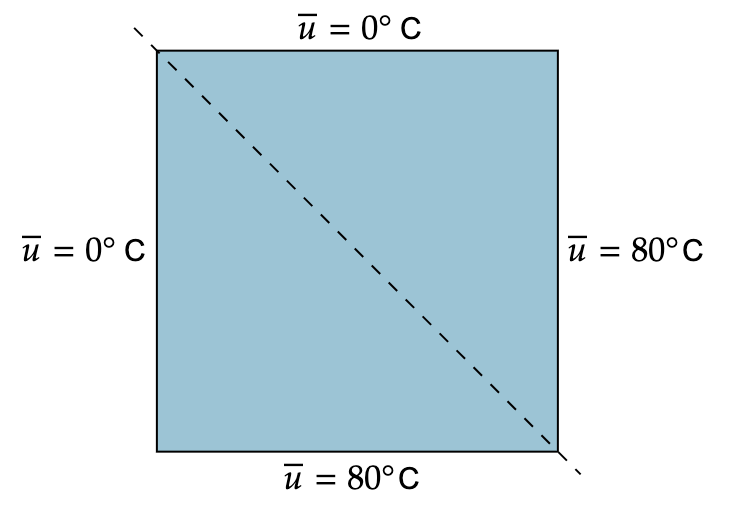
\includegraphics[width=0.6\textwidth]{Images/ab2/ab19.png}
    \caption{Simmetry with respect to the diagonal line.}
    \label{fig:ab19}
\end{figure}


